\documentclass[12pt,a4paper]{article}

% Package to include code
\usepackage{michel}
\usepackage{listings}
\usepackage{inconsolata}
\usepackage{color}

\usepackage{tikz}
\usetikzlibrary{trees}
\usepackage{pgfplots}
\lstset{language=Python}
\lstset{numbers=none, basicstyle=\ttfamily\footnotesize,
  numberstyle=\tiny,keywordstyle=\color{blue},stringstyle=\ttfamily,showstringspaces=false}
\lstset{backgroundcolor=\color[rgb]{0.95 0.95 0.95}}
\lstdefinestyle{numbers}{numbers=left, stepnumber=1,
  numberstyle=\tiny,basicstyle=\footnotesize, numbersep=10pt}
\lstdefinestyle{nonumbers}{numbers=none}
\lstset{
  breaklines=true,
  breakatwhitespace=true,
}

\newcommand*{\examplesPath}{../../examples}

% Font selection: uncomment the next line to use the ``beton'' font
%\usepackage{beton}

% Font selection: uncomment the next line to use the ``times'' font
%\usepackage{times}

% Font for equations
\usepackage{euler}


%Package to define the headers and footers of the pages
\usepackage{fancyhdr}



\title{Arithmetic expressions in Biogeme}
\author{Michel Bierlaire}
\date{\today}


\begin{document}


\begin{titlepage}
  \pagestyle{empty}

  \maketitle
  \vspace{2cm}

  \begin{center}
    \small Report TRANSP-OR 23xxxx \\ Transport and Mobility Laboratory \\ School of Architecture, Civil and Environmental Engineering \\ Ecole Polytechnique F\'ed\'erale de Lausanne \\ \verb+transp-or.epfl.ch+
    \begin{center}
      \textsc{Series on Biogeme}
    \end{center}
  \end{center}


  \clearpage
\end{titlepage}


The package Biogeme (\texttt{biogeme.epfl.ch}) is designed to estimate
the parameters of various models using maximum likelihood
estimation. It is particularly designed for discrete choice
models.

This document describes how Biogeme handles arithmetic expressions and
deals with potential numerical issues. The concepts have been
implemented in  \lstinline+cythonbiogeme 1.0.2+, used by
\lstinline+biogeme 3.2.13+.


\section{Introduction}\label{eq:intro}

The core of the Biogeme software package is the calculation of
formulas for each observation in a database. In estimation mode, the
formula is the log likelihood function. And its derivatives are
necessary for the optimization algorithm as well as the calculation of
useful statistics.  In simulation mode, the formulas are any indicator
that the analyst deeems useful to calculate (choice probabilities,
elasticities, etc.) We refer the reader to \citeasnoun{Bier18a} and
\citeasnoun{Bier23} for more details about the use of Biogeme for
model estimation and the calculation of indicators.


To allow the user to use Biogeme on a wide variety of model
specifications, the formulas are composed of elementary arithmetic
operations. These building blocks are organized in a complex tree structure, where each of them receives inputs from others, generates output, that is forwarded to the next layer.
For instance, the formula
\[
-x + \frac{\exp(y - 1)}{2}
\]
can be represented as illustrated in Figure~\ref{fig:tree}.

\begin{figure}[htb]
  \begin{center}
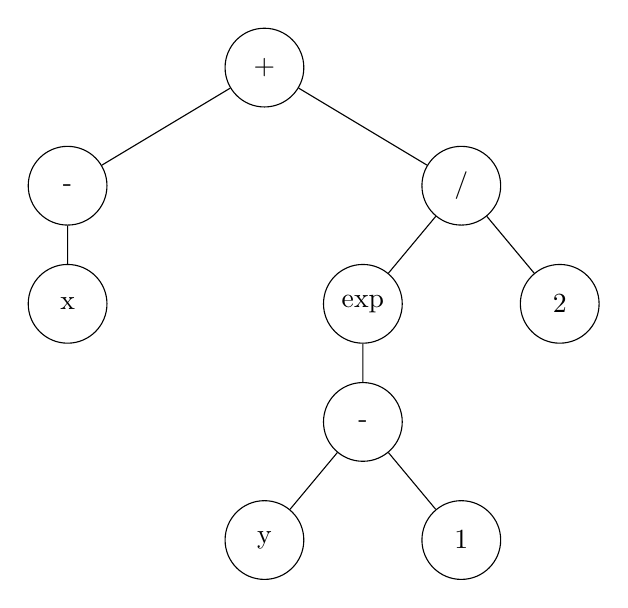
\begin{tikzpicture}[level distance=1.5cm,
  level 1/.style={sibling distance=5cm},
  level 2/.style={sibling distance=2.5cm},
  every node/.style={circle, draw, minimum size=1cm, inner sep=0pt, align=center}
  ]
  \node {+}
    child {
      node {-} 
      child {node {x}}
    }
    child {
      node {/}
      child {
        node {exp}
        child {
          node {-}
          child {node {y}}
          child {node {1}}
        }
      }
      child {node {2}}
    };
\end{tikzpicture}
  \end{center}
\caption{\label{fig:tree}Tree representation of a formula}
\end{figure}

Each node of the formula is associated with a specific simple
operation, and is in charge of calculating its value, and its
derivatives.


Computers are working with finite arithmetic. It means that computers
have limitations in the way they represent and operate on numbers due
to their finite hardware resources and the design of numerical
representations.  Therefore, the actual implementation of the
arithmetic operations are not necessarily an exact duplicate of their
mathematical equivalent, that consider a continuous space of real
numbers, that can take any value.

The objective of this document is to describe how each arithmetic expression is handled by Biogeme. 

\section{Numerical limits}

The computer representation of a real number is called a ``floating-point'' representation. It is divided into three parts. The values of the parameters below correspond to a 64-bit representation:
\begin{itemize}
\item A sign bit $s$, that indicates the sign of the number (0 for positive, 1 for negative).
\item An exponent $e$ covering $k=11$ bits, that represents the exponent of the number in a biased form. By bias, it is meant that negative and positive powers of two are possible. The bias $b$ is added to obtain a positive number. The bias is $b=2^{k-1}-1=1023$, so that the exponents range between -1022 to +1023.
\item A mantissa ($m$), using $p-1$ bits, where $p$ is the precision. 
\end{itemize}
So, for a 64-bit representation, $s+k+p-1=64$, so that $p=53$.
Therefore, the value of a floating point number is
\[
(-1)^s (1+m) 2^{e-b}.
\]

This representation allows for only a finite quantity of real numbers to be represented: $2^{64} \approx 10^{19}$ numbers. And this imposes numerical limits. In Python, it is possible to retrieve information about those limits using \lstinline+numpy+. If you type \lstinline+print(np.finfo(float))+, you obtain:
\begin{lstlisting}
Machine parameters for float64
---------------------------------------------------------------
precision =  15   resolution = 1.0000000000000001e-15
machep =    -52   eps =        2.2204460492503131e-16
negep =     -53   epsneg =     1.1102230246251565e-16
minexp =  -1022   tiny =       2.2250738585072014e-308
maxexp =   1024   max =        1.7976931348623157e+308
Nexp =       11   min =        -max
smallest_normal = 2.2250738585072014e-308   smallest_subnormal = 4.9406564584124654e-324
---------------------------------------------------------------  
\end{lstlisting}

In this document, we consider two of those limits. We denote $u$ the largest value that can be represented, that is
\[
u \approx 10^{308}.
\]
We also consider $\varepsilon$, the ``machine epsilon'', that is the difference between 1.0 and the next smallest representable float larger than 1.0. It is an important value, because it means that, for each $x < \varepsilon$, adding $x$ to 1 will provide 1 as a result:
\[
1 + x = 1.
\]
This may clearly lead to unpredictable behavior of numerical calculations. As mentioned in the output of \lstinline+numpy+, the value of the machine epsilon in 64-bit representation is
\[
\varepsilon \approx 10^{-16}.
\]
There is an empirical way to calculate this value, using the following script:
\begin{lstlisting}
epsilon = 1
while 1.0 + epsilon != 1.0:
    epsilon /= 2.0
epsilon *= 2.0
\end{lstlisting}

\section{Expressions}

Arithmetic expressions in Biogeme are based on the following principles.
\begin{itemize}
\item A \emph{valid} value is a value $-\sqrt{u} \leq x \leq \sqrt{u}$, that is a value between $-10^{154}$ and $10^{354}$.
\item Each arithmetic expression takes as input one or several valid values, and always returns a valid value.
\item A value $x$ such that $x \leq \sqrt{\varepsilon}$, that is $x \leq 10^{-8}$ is considered to be zero in continuous arithmetic.  
\end{itemize}

Suppose that we have an expression $\alpha$.
In order to make values valid in the sense described above, we define a validation function $v$ as follows:
\begin{equation}
\label{eq:validation}
v(\alpha) = \left\{
\begin{array}{ll}
  \sqrt{u} & \text{if } \alpha \geq \sqrt{u}, \\ 
  -\sqrt{u} & \text{if } \alpha \leq -\sqrt{u}, \\
  \alpha & \text{otherwise}.
\end{array}
\right.
\end{equation}

Based on those principles, we explicitly characterize how each
arithmetic expression is implemented in Biogeme. Each expression in
Biogeme is represented by an object of generic type
\lstinline+Expression+.



The document is organized by groups of expressions:
\begin{itemize}
\item Elementary expressions, including the numbers, the variables, the parameters, etc.
\item The unary expressions, accepting one input value.
\item The comparison expressions, accepting two input values, and used to compare two expressions.
\item Other binary expressions, accepting two input values.
\item The n-ary expressions, accepting more than two values.
\item The logit expression, implementing the logit model.
\end{itemize}



\subsection{Elementary expressions}

The elementary expressions are the building blocks of any expression. They correspond to the leaves of the tree representation, such as the one illustrated in Figure~\ref{fig:tree}.  

\begin{description}
\item[Numeric values] Numeric values are the most basic expressions. The syntax for numeric values is
  \begin{lstlisting}
    Numeric(x)
  \end{lstlisting}
  where \lstinline+x+ is the value. In most cases, the user does not need to use this syntax, as Biogeme tries to identify them automatically.
  If the value $x$ is not valid, in the sense defined above, an exception is triggered.
\item[Variables] Variables are refering to the columns of the data set:
  \begin{lstlisting}
    Variable('name_of_the_variable')
  \end{lstlisting}
  This expression simply returns the value of the corresponding variable for the current row. No specific validity check is performed for the sake of computational efficiency.
\item[Parameters] Parameters must be estimated from data. Their first values is defined by the user. There are two categories of parameters. Free parameters are updated by the optimization algorithm.
  Fixed parameters are not.
  The syntax for parameters is
  \begin{lstlisting}
    Beta('name_of_the_parameter', x_0, ell, u, fixed)
  \end{lstlisting}
  where \lstinline+x_0+ is the initial value of the parameter,
  \lstinline+ell+ is the lower bound on the parameter, \lstinline+u+ is the upper bound on the parameter, and \lstinline+fixed+ specifies if the parameter must be fixed (\lstinline+fixed=1+) of free (\lstinline+fixed=0+).
  If the value \lstinline+x_0+, \lstinline+ell+ or \lstinline+u+  is not valid, in the sense defined above, an exception is triggered.
\item[Random variable] A random variable is used in the context of numerical integration.
\item[Draws] Random draws are used in the context of Monte-Carlo integration. 

\end{description}

Biogeme calculates derivatives with respects to ``literals'', that is, variables and parameters. In the following, we denote by $x_i$ and $x_j$ the literals that are involved in the derivatives.
Obviously, we have
\[
\frac{\partial x_i}{\partial x_i}=1, \;
\frac{\partial x_i}{\partial x_j}=0, \;
\]
and
\[
\frac{\partial^2 x_i}{\partial x_i^2}=\frac{\partial^2 x_i}{\partial x_i \partial x_j} = 0. 
\]


\subsection{Unary expressions}

Unary expressions take one value as input. Like any expression, they return a value and the derivatives.
\begin{description}
\item[Unary minus] If $\alpha$ is the input value, it returns $f(\alpha)=-\alpha$. The syntax is simply
  \begin{lstlisting}
    -alpha
  \end{lstlisting}
  As $\alpha$ is a valid value, so is $f(\alpha)$. The derivatives are:
  \[
  \frac{\partial f}{\partial x_i} = - \frac{\partial \alpha}{\partial x_i}
  \]
  and
  \[
  \frac{\partial^2 f}{\partial x_i \partial x_j} = - \frac{\partial \alpha}{\partial x_i \partial x_j}.
  \]
\item[Exponential] Let $\alpha$ be the input value.
  \begin{itemize}
  \item  If $\alpha \leq \ln(\sqrt{u})$, then
    \[
    f(\alpha)=e^\alpha.
    \]
    Also, the derivatives are
    \[
    \frac{\partial f(\alpha)}{\partial x_i} = v\left(e^\alpha \frac{\partial \alpha}{\partial x_i}\right),
    \]
    and
    \[
    \frac{\partial^2 f(\alpha)}{\partial x_i \partial x_j} = v\left(e^\alpha (\frac{\partial \alpha}{\partial x_i}\frac{\partial \alpha}{\partial x_j} + \frac{\partial^2 \alpha}{\partial x_i \partial x_j})\right),
    \]
    where $v$ is the validation function \req{eq:validation}.
  \item If $\alpha > \ln(\sqrt{u})$, then
    \[
    f(\alpha) = \frac{\partial f(\alpha)}{\partial x_i} = \frac{\partial^2 f(\alpha)}{\partial x_i \partial x_j} = \sqrt{u}.
    \]
  \end{itemize}

\item[Logarithm] Let $\alpha$ be the input value.
  \begin{itemize}
  \item If $\sqrt{\varepsilon} \leq \alpha \leq e^{\sqrt{u}}$, we define
    \begin{align*}
    f(\alpha)& =\ln(\alpha), \\ 
    \frac{\partial f(\alpha)}{\partial x_i} &= v\left(\frac{1}{\alpha} \frac{\partial \alpha}{\partial x_i}\right), \\
    \frac{\partial^2 f(\alpha)}{\partial x_i \partial x_j} &=
    v\left(-\frac{1}{\alpha^{2}}
    \frac{\partial \alpha}{\partial x_i}
    \frac{\partial \alpha}{\partial x_j }
    + \frac{1}{\alpha}
    \frac{\partial^2 \alpha}{\partial x_i \partial x_j}
      \right).
    \end{align*}
  \item If $\alpha > e^{\sqrt{u}}$, we define
    \[
    f(\alpha) = \frac{\partial f(\alpha)}{\partial x_i} = \frac{\partial^2 f(\alpha)}{\partial x_i \partial x_j} = \sqrt{u}.
    \]
  \item If $0 \leq  \alpha < \sqrt{\varepsilon}$, we define
    
  \end{itemize}
 
\end{description}
  



bioExprLogzero.h
bioExprDerive.h
bioExprIntegrate.h / bioExprGaussHermite.h
bioExprMontecarlo.h
bioExprNormalCdf.h
bioExprPanelTrajectory.h
\subsection{Comparison expressions}
bioExprEqual.h
bioExprNotEqual.h
bioExprGreater.h
bioExprGreaterOrEqual.h
bioExprLess.h
bioExprLessOrEqual.h
\subsection{Binary expressions}
bioExprPlus.h
bioExprMinus.h
bioExprTimes.h
bioExprDivide.h
bioExprPower.h
bioExprMin.h
bioExprMax.h
bioExprAnd.h
bioExprOr.h
\subsection{n-ary expressions}
bioExprMultSum.h
bioExprElem.h
bioExprLinearUtility.h
\subsection{Logit expressions}
bioExprLogLogit.h
bioExprLogLogitFullChoiceSet.h




%%% Investigate where these functions are used, if at all.
%bioExprNormalPdf.h
%bioExprSum.h





\bibliographystyle{dcu}
\bibliography{transpor}


\end{document}
